\chapter{User Documentation} % User guide
\label{ch:user}

The User Documentation contains a basic overview of the application, the system requirements, an installation guide and instructions on how to use the application.

\section{System requirements}
\subsection{Hardware requirements}
The application itself is lightweight and does not require strong hardware. It however requires a Kubernetes cluster to work on, therefore Kubernetes' system requirements apply to it. It is worth to note, that serving tens of thousands if not more users (which Kubernetes clusters are intended for) needs multiple strong server machines. For testing purposes, a single pc or laptop will suffice. \\

There are two kind of Kubernetes nodes: master and worker nodes. In every cluster, there is one master node, which controls the workers. There is no limit on worker count. It is possible to run a master and a worker node on one computer to avoid needing multiple machines.
\bigbreak

\newpage
\noindent
Hardware requirements of Kubernetes master nodes:
\begin{itemize}
	\item CPU: At least two cores @ 1 GHz. X86-64 recommended, ARM64 might work, but it is untested. 
	\item RAM: At least 2 GB of free memory.
	\item Disk space: At least 2 GB recommended for the tooling (k8s-core, cert-updater, fluentd, kube-addon-manager, rescheduler, network, etcd, proxy, kubelet).
\end{itemize}

\noindent
Hardware requirements of Kubernetes worker nodes:
\begin{itemize}
	\item CPU: At least one core @ 1 GHz. X86-64 recommended, ARM64 might work, but it is untested. 
	\item RAM: At least 700 Mb of free memory.
	\item Disk space: At least 1 GB recommended for the tooling (fluentd, dns, proxy, network, kubelet).
\end{itemize}

\newpage
\subsection{Software requirements}
While Kubernetes runs on Windows as well as on Linux, generally most servers will run the latter, and a core part of the application - the eBPF programs - also run in the Linux kernel. Therefore, Linux is required and while the code might compile on Windows or macOS, it certainly will not run on them.\\
Another thing worth mentioning is that eBPF requires a fairly new kernel to run as it is a bleeding edge technology. The development took place on a computer running Manjaro 20.1.1 with Linux 5.10.15 kernel.
\bigbreak

\noindent
Software requirements of the application:
\begin{itemize}
	\item Linux with Kernel~\cite{linux-kernel} 5.10 or newer
	\item Kubernetes~\cite{kubernetes} v1.20 or newer, K3S~\cite{k3s} is recommended for \underline{\gls{on-premises}} clusters
	\item Clang~\cite{clang} 10.0 or newer
	\item BPF tools~\cite{bpf-1}
	\item LibBPF~\cite{libbpf}
	\item Go~\cite{go} 1.15 or newer
\end{itemize}

\newpage
\section{Overview}
\begin{figure}[H]
	\centering
	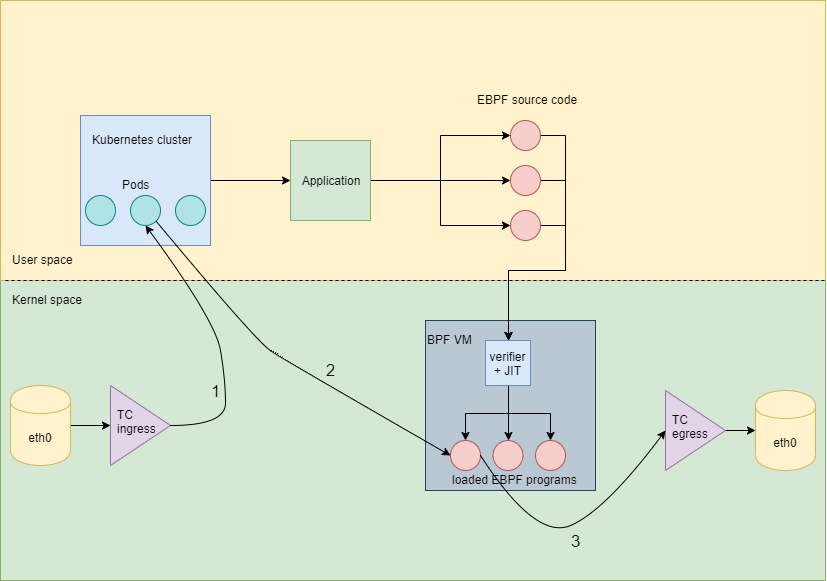
\includegraphics[width=\textwidth]{images/architecture.png}
	\caption{Application architecture}
	\label{fig:app-arch}
\end{figure}
Simply put, the application manages the traffic flowing through a Kubernetes cluster according to a set of rules. These rules can be as simple as applying a bandwidth limit, or dropping given packets. They can also be much more complex through user defined programs, if required.
\bigbreak

The center of operation is an executable written in Golang that uses the Kubernetes API to constantly monitor the state of the cluster. On startup, it fetches all Kubernetes services and pods, reading their metadata to decide if a limit should be set on them. All limits are applied on the pods themselves, even service ones. Services are linked to a set of pods, their limits are inherited by the pods, though if a pod has colliding limit, the pod-level one is applied.
\bigbreak

Since a pod is not one process, but an abstraction above closely related ones, it is not possible to simply control their traffic. Instead, even though they are treated as one unit, the underlying processes are iterated and all of them are set to the same limits.
\bigbreak

\noindent
The process of applying limits is the following:
\texttt{
\begin{enumerate}
	\item Finding the pod on which the limit gets applied
	\item Iterate over the processes of the pod
	\begin{enumerate}
    	\item Get the cgroup of the process
    	\item Compile a custom-tailored eBPF program using pre-written templates
    	\item Load the eBPF program into the Linux kernel
    	\item Attach the eBPF program to the cgroups' socket buffer hooks
    \end{enumerate}
	\item Save the limit info of the pod
\end{enumerate}
}
\noindent
The reason each pod is required to compile its own eBPF program in \textbf{step 2B} is due to an inherent property of the eBPF system: it does not support parametrizing the programs. This is bypassed by the application using C macros that are set compile-time; further info about this in the Developer Documentation part.

\newpage
\section{Installation guide}
For development, Manjaro 20.1.1 with Linux 5.10.15 kernel was used. The Installation Guide will also be based on this.

\subsection{Initial setup}
\subsubsection{Linux kernel version}
The first step is to ensure a new enough linux kernel is running on the machine. The features used in the eBPF programs require a kernel version newer than 5.10. To check, open a terminal and run
\begin{verbatim}
$ uname -r 
\end{verbatim}
This outputs the version of the currently running kernel. If the kernel version is too old, a simple way to update it is to use the Manjaro Settings Manager. After opening it, click on \texttt{Kernel}. It will show a list of kernels available to be installed. Choose a version of 5.10 or over. Click \texttt{Install}, then restart the machine and check the version again.

\subsubsection{Required software}
If the kernel is up to date, the next step is to install the required tools that will be used to compile the Go application, the eBPF programs - which, by the way are written in a subset of C - and load them into the kernel. The easiest way is to open a terminal and run
\begin{verbatim}
$ sudo pacman -S base-devel go clang bpf libbpf
\end{verbatim}
\noindent
This will install every required piece of software, namely:
\begin{enumerate}
    \item \texttt{base-devel}: This is a basic bundle of software that is used by virtually everything else.
    \item \texttt{go}: The Golang compiler and tooling. Required for compiling the application itself.
    \item \texttt{clang}: A C compiler used to generate the object files from C source code.
    \item \texttt{bpf}, \texttt{libbpf}: These utilities are used to load the object files into the kernel.
\end{enumerate}


\subsection{Kubernetes Cluster}
Kubernetes - being a complex software bundle - requires the help of guides to install. Since it is a core requirement, a short one is included in the thesis.\\
The project uses K3S due to the ease of setup, as it bundles a CNI (Flannel) and Ingress controller (Traefik ~\cite{traefik}). These require little to no configuration - something that is a severe problem when using raw kubeadm, kubelet and kubectl utilities.

\subsubsection{Using the bundled executable}
The easiest way to set up the cluster is to simply run the bundled executable. This is located in the  \textit{k3s} folder. Normally, including executables is to be avoided; in this case, the main motivations were a simple setup procedure and the fact that at the time of writing the application, the latest K3S releases were not capable of using Cgroup v2. The fix was already done, a release had yet to be published.

\noindent
To start the Kubernetes cluster, open a terminal and run
\begin{verbatim}
$ sudo k3s/run.sh
\end{verbatim}

\noindent
This will start the master node with an additional worker node. The ramp-up period depends on the speed of the machine, generally, half a minute should be enough for it.

\subsubsection{Installing natively}
A more elaborate and recommended way to install the Kubernetes cluster is to follow the official way. This will set up a service on the machine that will by default start up on boot. This spares the burden of having to manually start the executable each time. To install the K3S service, open a terminal and run
\begin{verbatim}
$ curl -sfL https://get.k3s.io | sh -
\end{verbatim}

\noindent
The install script will automatically set up everything required to run the service, this usually takes around a minute or so. After installation, the cluster will automatically start to run, creating a master and a worker node. Ensure the service is running using
\begin{verbatim}
$ systemctl status k3s.service
\end{verbatim}

\subsubsection{Configuring the cluster}
Configuring the cluster itself is depenent on intent. For development or production clusters, this part can be skipped entirely as it follows the configuration of the example bundled service. \\

The example service is kept as minimal as possible to keep complexity down. The server binary itself listens on \texttt{port 80}, and the \texttt{config.yml} file contains directives to run this executable. A pod is created to serve as a platform the executable can run on, and a service is masking the pod towards the ingress controller. This will be explained further in the Development Documentation. Traefik is used as an ingress controller (a reverse proxy), to interface the service to the real world. All these elements reside inside the thesis-ns namespace to differentiate them from everything else and keep things tidy. \\

\noindent
To apply the configuration, run the
\begin{verbatim}
$ sudo k3s/k3s kubectl apply -f k3s/config.yml
\end{verbatim}
or 
\begin{verbatim}
$ sudo k3s kubectl apply -f k3s/config.yml
\end{verbatim}
\noindent
command in a terminal depending whether you used the executable or installed the k3s service. \\

\label{sec:k3syaml}By default, K3S will put the kubeconfig file - which will be needed later - into the \texttt{/etc/rancher/k3s/config.yaml} folder. It is recommended to move this into the home directory for ease of use, before it is forgotten. This can be done by running
\begin{verbatim}
$ cp /etc/rancher/k3s/config.yaml ~/.kube/config
\end{verbatim}

\newpage
The last thing to configure is the cgroup v2. It is usually not enabled by default. To do so, the following steps can be taken.
\begin{enumerate}
	\item \texttt{\$ sudo nano /etc/default/grub}
	\item Append \texttt{cgroup\_no\_v1=net\_prio,net\_cls systemd.unified\_cgroup\_hierarchy=1} to the end of both \texttt{GRUB\_CMDLINE\_LINUX\_DEFAULT} and \texttt{GRUB\_CMDLINE\_LINUX} lines.
	\item Save and exit
	\item \texttt{\$ sudo update-grub}
	\item Reboot the machine
\end{enumerate}

After rebooting, make sure it is actually set up correctly. It can be checked using the following command.
\begin{verbatim}
$ mount | grep cgroup
\end{verbatim}

The output should resemble \texttt{cgroup2 on /sys/fs/cgroup type cgroup2 (rw,nosuid,nodev,noexec,relatime)}.

\newpage
\subsection{Compiling and running the executable}
\subsubsection{Compiling the application}
The application itself is written in Golang and can be compiled and run either in terminal, by systemd~\cite{systemd} daemon or an \underline{\gls{ide}} of your choice (Goland~\cite{goland} is recommended).

The newest dependency management software of Golang is called Go modules. As the name states, projects are organized into a coherent entity called a module, which other modules can depend on. A dependency tree is built from these, with the current module at its root. This project also uses go modules.

\noindent
Go modules have some rules that help to standardize compilation and program entry points. To compile the application, simply run
\begin{verbatim}
$ cd ebpf_loader && go build -o podmgr .
\end{verbatim}

\noindent
This will create an executable in the current folder that can be then directly run by stating
\begin{verbatim}
$ sudo ./podmgr
\end{verbatim}
\noindent
The application always requires root privileges because it calls commands that interact with the system directly, such as the loading of eBPF programs into the kernel and managing cgroups.

\subsubsection{Adding a daemon}
It is possible to create a daemon for the application which would start automatically upon boot. Nowadays, the most popular init system is systemd, but sysvinit, OpenRC and upstart daemon are also supported.

To make a systemd daemon, create a .service file in the \texttt{/etc/systemd/system} folder, and set the ExecStart parameter to the executable file.

\newpage
\section{Using the application}
The application uses the Kubernetes API (Application Programming Interface) to continuously monitor the cluster. This API requires authentication, provided by the kubeconfig file. By convention, this file resides in the \texttt{~/.kube/config} directory. \underline{\hyperref[sec:k3syaml]{Section 2.3.2}} explains where this file is located when using a K3S installation.

Alternatively, the location of the kubeconfig file can be passed to the application through the kubeconfig command line flag. This is useful when the location of the file can not be changed.

\subsection{Effect level}
There are several ways the application can affect the cluster, however a common thing between them is that they all act on pod level regardless how they are configured. \\

There are two ways to apply the rules. The first one is directly applying them to the pods, and the second way is to apply them to services. Services are abstractions over multiple pods, and they can be used to have them all get the same settings without having to repeat the rule.

When both service- and pod level rules are set, the pod level ones overrule the service ones. In all other cases, trivially only the set rules are applied.

The rules themselves can be applied through appending metadata in the yaml (YAML Ain't Markup Language, a type of config) files that describe Kubernetes components. \\

It is desirable to avoid using multiple rules on one pod; though it is possible to make them work together, collisions or conflicts may still happen. As a rule of thumb, the less logic is in the way of the transmitted data, the faster the connection is. 

\newpage
\subsubsection{Adding a pod level rule}
Pod level rules are directly set on the pods. Simply add a metadata member called \texttt{annotations}, then list the rules to be applied. Deployments are also supported, in this case the annotations go into the template metadata.

\lstset{caption={Examle yaml file describing a pod with a 10 Mbps bandwidth limit}, label=yamlex2}
\begin{lstlisting}[language={C++}]
apiVersion: v1
kind: Pod
metadata:
  name: static-web
  labels:
    app: myapp
  annotations:
    bandwidth: "10 mbps egress"
spec:
  ...
\end{lstlisting}

\subsubsection{Adding a service level rule}
Service level rules are - like the name says - set on services that mask the pods. This allows the rules to be applied to several pods without repetition of the rule. Add a metadata member called \texttt{annotations}, then list the rules to be applied.
\lstset{caption={Examle yaml file describing a service with a 10 Mbps bandwidth limit}, label=yamlex3}
\begin{lstlisting}[language={C++}]
apiVersion: v1
kind: Service
metadata:
  name: myservice
  annotations:
    bandwidth: "10 mbps egress"
spec:
  ...
\end{lstlisting}

\newpage
\subsection{Using the Bandwidth manager}
The bandwidth manager is a built-in rule that acts as a low-pass filter by setting a maximum bandwidth that a pod can use. This can be useful for a variety of purposes.
\begin{itemize}
	\item Testing how a specific service reacts to low-bandwidth environments. 
	\item Applying QoS (Quality of Service) policies
	\item Keeping the network load below a set value (cloud providers often bill network usage)
\end{itemize}

\noindent
Internally, the bandwidth manager uses TBF (Token Bucket Filter) to drop packages that do not fit in the bandwidth. These dropped packets by themselves are already enough to maintain the limit, but when using TCP - and generally, web services use TCP - it will also throttle back the speed of the connection, sending packets slower and further regulating the limit.

\subsubsection{Adding a bandwidth limit}
To add a bandwidth limit to a pod or service, open the yaml config file of it, and add a \texttt{bandwidth} key in the annotation section.

\lstset{caption={Example bandwidth limit of 10 Mbps}, label=yamlex4}
\begin{lstlisting}[language={C++}]
...
metadata:
  annotations:
    bandwidth: "10 mbps egress"
...
\end{lstlisting}
\noindent
The value of the key follows the pattern of

\begin{itemize}
	\item speed - \texttt{integer}, the maximum bandwidth.
	\item unit - \texttt{string}, could be any of \texttt{bps}, \texttt{kbps} and \texttt{mbps}.
	\item interface - \texttt{string}, either \texttt{ingress} or \texttt{egress}.
\end{itemize}

\subsection{Using the Loss Manager}
The Loss manager is also a built-in rule, dropping packets randomly according to some settings. The default behavior uses uniform distribution and the dropped packet ratio can be given as a percentage. For example, a loss of 5\% would drop every twentieth packet on average - of course, this varies due to the nature of the random numbers. The loss manager can be an useful tool in several cases.
\begin{itemize}
	\item Testing how a specific service reacts to high-congestion environments. 
	\item Simulating high packet loss, for example caused by poor Wi-Fi reception.
	\item Simulating misconfigured networks or software.
\end{itemize}

\noindent
The loss manager uses a PRNG (pseudorandom number generator) supplied by an BPF utility which supplies 32 bit long data. This is then converted to percentage by taking modulo 100 of it. The output can then be directly compared.

\subsubsection{Adding a loss ratio}
To add a loss ratio to a pod or service, open the yaml config file of it, and add a \texttt{loss} key in the annotation section.

\lstset{caption={Example loss of 2 percent}, label=yamlex5}
\begin{lstlisting}[language={C++}]
...
metadata:
  annotations:
    loss: "uniform egress 2%"
...
\end{lstlisting}

\noindent
The value of the key follows the pattern of

\begin{itemize}
	\item distribution - \texttt{string}, either \texttt{uniform} or \texttt{exponential}.
	\item interface - \texttt{string}, either \texttt{ingress} or \texttt{egress}.
	\item threshold - \texttt{string}, for uniform distribution, a \texttt{percentage}, for exponential, a \texttt{value in [0, 1000]}.
\end{itemize}

\subsection{Using custom programs}
Custom programs can be written to further extend the functionality of the application. 
This enables users to police the in- and outbound traffic as they see fit without having tho write a surrounding mechanism that controls the loading and unloading of these programs. These custom programs can control traffic based on virtually anything that conforms to the eBPF rules.

\subsubsection{Writing the eBPF program}
The eBPF programs are written in a subset of C. Specific rules apply to the code, this is further explained in \underline{\hyperref[sec:ebpfrules]{Section 3.2.2}}.
More information about writing these programs can be found in Cilium's eBPF reference guide~\cite{ebpfref}.

Note, the interface (ingress, egress) is automatically applied as the \texttt{INTERFACE} macro in these programs.

\subsubsection{Applying the rules}
To add a custom program, open the yaml config file of the pod and add the \texttt{ebpf-limit} key in the annotation section.

\lstset{caption={Example of a custom program applied}, label=yamlex1}
\begin{lstlisting}[language={C++}]
...
metadata:
  annotations:
    ebpf-limit: "dropper egress -DDROP=1"
...
\end{lstlisting}

\noindent
The value of the key follows the pattern of

\begin{itemize}
	\item name - \texttt{string}, the name of the program.
	\item interface - \texttt{string}, either \texttt{ingress} or \texttt{egress}.
	\item parameters - these are passed to Clang during compilation, useful for setting macros.
\end{itemize}


The macros follow the pattern of \texttt{-DNAME=value} where -D is constant, NAME is the name of the macro and the value is what the name gets replaced with.

\subsection{Shutting down the application}
To quit, simply press Ctrl + C in the terminal or if a systemd daemon is used, issue the following command:
\begin{verbatim}
$ sudo systemctl stop application
\end{verbatim}

The application will automatically remove the limits, detach all eBPF programs and delete the build artifacts.